\begin{center}
\resizebox{\linewidth}{!}{%
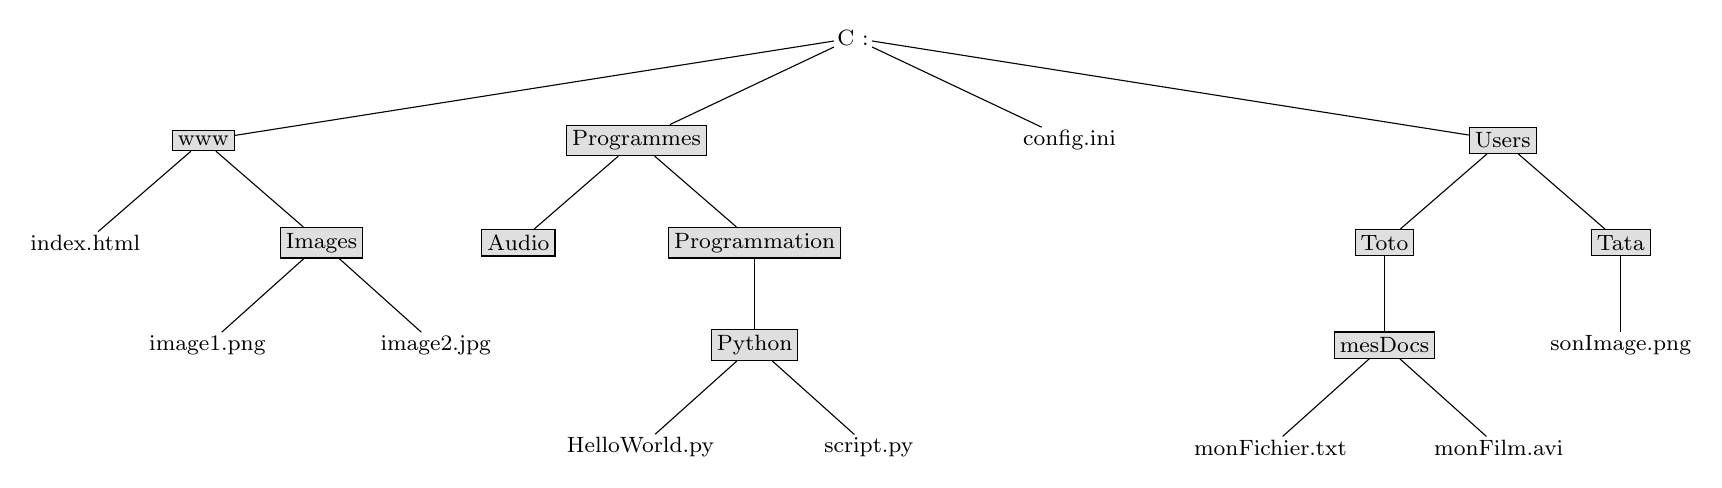
\begin{tikzpicture}[font=\footnotesize,
 d/.style={draw,fill=gray!25,inner sep=2pt},f/.style={inner sep=1pt},
 level distance=1.3cm,
 level 1/.style={sibling distance=5.5cm},level 2/.style={sibling distance=3cm},level 3/.style={sibling distance=2.9cm}]
\node[f] {C :}
 child {node[d] {www}
   child {node[f] {index.html}}
   child {node[d] {Images} child {node[f] {image1.png}} child {node[f] {image2.jpg}}}}
 child {node[d] {Programmes}
   child {node[d] {Audio}}
   child {node[d] {Programmation} child {node[d] {Python} child {node[f] {HelloWorld.py}} child {node[f] {script.py}}}}}
 child {node[f] {config.ini}}
 child {node[d] {Users}
   child {node[d] {Toto} child {node[d] {mesDocs} child {node[f] {monFichier.txt}} child {node[f] {monFilm.avi}}}}
   child {node[d] {Tata} child {node[f] {sonImage.png}}}};
\end{tikzpicture}}

\small Les cadres grisés sont des dossiers.
\end{center}
